\documentclass[12pt]{article}
\usepackage{preamble}

\pagestyle{fancy}
\fancyhead[LO,LE]{Дополнительные главы \\ высшей математики}
\fancyhead[CO,CE]{18.10.2024}
\fancyhead[RO,RE]{Лекции Далевской О. П.}

\fancyfoot[L]{\scriptsize исходники найдутся тут: \\ \url{https://github.com/pelmesh619/itmo_conspects} \Cat}

\begin{document}
    \begin{MyTheorem}
        \Ths Если ряд $\sum_{n = 1}^\infty u_n(x) \ (u_n(x) \in C_{[a, b]})$ мажорируем в $D = [a, b]$, то 
        его сумма $S_x$ непрерывна на $[a, b]$
    \end{MyTheorem}

    \begin{MyProof}
        $\Box$

        $S(x)$ непрерывна на $x \in [a, b] \Longleftrightarrow \Delta S \underset{\Delta x \to 0}{\rightarrow} 0$

        $\Delta S(x) = S(x + \Delta x) - S(x), \ S(x) = S_n(x) + r_n(x)$

        $\Delta S_n(x) = S_n(x + \Delta x) - S_n(x)$

        $\Delta S = S(x + \Delta x) - S(x) = S_n(x + \Delta x) + r_n(x +  \Delta x) - S_n(x) - r_n(x)$

        $\Delta S(x) = \Delta S_n + r_n(x + \Delta x) - r_n(x)$

        $|\Delta S(x)| \leq |\Delta S_n| + |r_n(x + \Delta x)| + |r_n(x)|$

        Ряд $\sum_{n = 1}^\infty u_n(x)$ мажорируем $\Longleftrightarrow \exists$ сходящийся $\sum_{n = 1}^\infty \alpha_n \ \Big| \ |u_n(x) \leq \alpha_n|$
    
        Тогда $\forall \varepsilon > 0 \ \exists N = N(\varepsilon) \ | \ |r_n(x)| < \frac{\varepsilon}{3}$

        и $\forall \varepsilon > 0 \ \exists N = N(\varepsilon) \ | \ |r_n(x + \Delta x)| < \frac{\varepsilon}{3}$ (так как $N$ не зависит от $x$; $x + \Delta x \in [a, b]$) 
    
        $\Delta S_n = S_n(x + \Delta x) - S(x) = u_n(x + \Delta x) - u(x) + \dots + u_n(x + \Delta x) - u_n(x)$ - конечная сумма непрерывна

        Сама $S_n(x)$ непрерывна, тогда $\forall \varepsilon > 0 \ $ (при фиксированном $N$) $\exists \delta > 0 \ | \ |\Delta S_n(x)| < \frac{\varepsilon}{3}$ при $|\Delta x| < \delta$

        \bgroup
        \setlength\tabcolsep{1.5pt}
        \begin{tabular}{ccl}
            Итак: $\forall \varepsilon > 0 \ \exists N = N(\varepsilon)$ и $\delta > 0 \ | \ \underset{|\Delta x| < \delta}{\forall x \in D}$ & & $|\Delta S_n(x)| < \frac{\varepsilon}{3}$ \\
            
            & $+$ & $|r_n(x + \Delta x)| < \frac{\varepsilon}{3}$ \\ 
            
            & $+$ & $|r_n(x)| < \frac{\varepsilon}{3}$ \\

            & $=$ & $|\Delta S(x)| < \varepsilon$
        \end{tabular}
        \egroup

        То есть $S(x) \in C_{[a, b]}$

        $\Box$
    \end{MyProof}

    \Nota Не все равномерно сходящиеся мажорируются, но у всех $S(x)$ непрерывна

    Это позволяет определить $\int_{x_0}^y S(x) dx$, а если $S(x) \in C^\prime_{[a, b]}$, то и $\frac{dS(x)}{dx}$

    \begin{MyTheorem}
        \Ths Если ряд мажорируется на $[a, b]$ и $u_n(x)$ непрерывна на $[a, b]$, то определен $\int_{x_0}^y S(x)dx$ и 
        $\int_{x_0}^x S(x)dx  = \sum_{n = 1}^\infty \int_{x_0}^x u_n(x) dx$
    \end{MyTheorem}

    \begin{MyProof}
        $\Box$

        $S(x) = S_n(x) + r_n(x) = u_1(x) + u_2(x) + \dots + u_n(x) + r_n(x)$ - конечное число слагаемых из непрерывных функций
        ($r_n(x)$ как хвост равномерно сходящегося ряда)

        Тогда для $x_0, x \in [a, b] \quad \int_{x_0}^x S(x) = \sum_{k = 1}^n \int_{x_0}^x u_k(x) dx + \int_{x_0}^x r_n(x) dx$ - это будет
        верно, если $\int_{x_0}^x r_n(x) dx \underset{n \to \infty}{\longrightarrow} 0$

        По свойству интегралов $\left|\int_{x_0}^x r_n(x) dx\right| \leq \int_{x_0}^x |r_n(x)| dx$

        $\left|\int_{x_0}^x r_n(x) dx\right| \leq \int_{x_0}^x |r_n(x)| dx < \int_{x_0}^x \varepsilon_n dx = \underset{\varepsilon_n \to 0}{\varepsilon_n (x - x_0)}$ ($x, x_0$ - фикс.)

        То есть $\lim_{n \to \infty} \int_{x_0}^x r_n(x) dx = 0$

        $\lim_{n \to \infty} \int_{x_0}^x S(x) dx = \lim_{n \to \infty} \sum_{k = 1}^n \int_{x_0}^x u_k(x) dx + \lim_{n \to \infty} \int_{x_0}^x r_n(x) dx$

        $\int_{x_0}^x S(x) dx = \sum_{n = 1}^\infty \int_{x_0}^x u_n(x) dx$

        $\Box$
    \end{MyProof}

    \Nota Почленно интегрируются не просто равномерно сходящиеся, а мажорируемые, иначе остаток необязательно стремится к 0

    \begin{MyTheorem}
        \Ths $\sum_{n = 1}^\infty u_n(x)$ мажорируем на $[a, b]$ и $u_n(x) \in C^\prime_{[a, b]}$

        Тогда $S^\prime(x) = \sum_{n = 1}^\infty u^\prime_n(x)$
    \end{MyTheorem}

    
    \begin{MyProof}
        $\Box$

        Пусть $g(x) = \sum_{n = 1}^\infty u^\prime_n(x)$. Докажем, что $g(x) = S^\prime(x)$

        $\int_{x_0}^x g(x)dx = \int_{x_0}^x \left(\sum_{n = 1}^\infty u^\prime_n(x)\right) dx = \sum_{n = 1}^\infty 
        \left(\int_{x_0}^x u_n^\prime (x)dx\right) = u_1(x) \Big|_{x_0}^x + u_2(x) \Big|_{x_0}^x + \dots$

        $ = (u_1(x) - u_1(x_0)) + (u_2(x) - u_2(x_0)) + \dots = S(x) - S(x_0)$ - разность сходящихся рядов

        $\int_{x_0}^x g(x) dx = S(x) - S(x_0) \Longrightarrow \left(\int_{x_0}^x g(x) dx\right)^\prime = g(x) = S^\prime(x)$

        $\Box$
    \end{MyProof}

    \subsection{2. Степенные ряды}

    \Def $\sum_{n = 0}^\infty c_n(x - x_0)^n, \ c_n \in \Real, x_0 \in \Real$ - степенной ряд с центром $x_0$ (в точке $x_0$, по степеням $(x - x_0)$)

    \Nota В частности $\sum_{n = 1}^\infty c_n x^n$ - степенной с центром в $x_0 = 0$

    $\sum_{n = 0}^\infty c_n(x - x_0)^n$ легко сводится заменой $x - x_0 = t$ к $\sum_{n = 0}^\infty c_n t^n$

    \begin{MyTheorem}
        \ThNs{Абеля} 

        1) $\sum_{n = 0}^\infty c_n x^n$ сходится в точке $x_1$. Тогда ряд сходится для любого $x$, который $|x| < |x_1|$

        2) $\sum_{n = 0}^\infty c_n x^n$ расходится в точке $x_2$. Тогда ряд расходится $\forall x \ |x| > |x_2|$
    \end{MyTheorem}

    \begin{MyProof}
        $\Box$

        1) В точке $x_1$ $\sum_{n = 0}^\infty c_n x_1^n = c_0 + c_1 x_1 + c_2 x_1^2 + \dots$ - числовой ряд, сходящийся

        В точке $x \ (|x| < |x_1|) \quad \sum_{n = 0}^\infty c_n x^n = c_0 + c_1 x + c_2 x^2 + \dots = 
        c_0 + c_1 x_1 \frac{x}{x_1} + c_1 x_1^2 \frac{x^2}{x_1^2} + \dots$ 

        Для этого ряда докажем абсолютную сходимость

        $\sum_{n = 0}^\infty |c_n x^n| = |c_0| + |c_1 x_1| \left|\frac{x}{x_1}\right| + |c_1 x_1^2| \left|\frac{x^2}{x_1^2}\right| + \dots$

        При этом ряд $\sum_{n = 0}^\infty c_n x_1^n$ сходится $\Longrightarrow \exists M > 0 \ : \ |c_n x_1^n| \leq M$

        И $\left|\frac{x^k}{x_1^k}\right| < 1$, так как $|x| < |x_1|$

        Тогда $|c_0| + |c_1 x_1| \left|\frac{x}{x_1}\right| + |c_1 x_1^2| \left|\frac{x^2}{x_1^2}\right| + \dots + |c_k x_1^k| \left|\frac{x^k}{x_1^k}\right| < 
        M\left(1 + \left|\frac{x}{x_1}\right| + \left|\frac{x}{x_1}\right|^2 + \dots + \left|\frac{x}{x_1}\right|^k\right)$ - геометрическая прогрессия с $|q| < 1$

        Таким образом $\sum_{n = 0}^\infty |c_n x^n| \sim M\sum_{n = 0}^\infty \left|\frac{x}{x_1}\right|^n$, который сходится

        Ряд $\sum_{n = 0}^\infty c_n x^n$ абсолютно сходится (и равномерно?)

        б) От противного, используя пункт а)

        $\Box$
    \end{MyProof}

    \smallvspace

    \begin{minipage}{\textwidth}
        \begin{wrapfigure}{r}{0pt}
            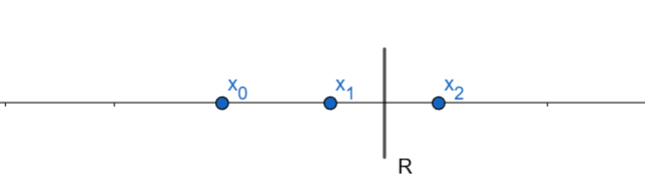
\includegraphics[width=0.4\textwidth]{addchapters1/images/addchapters1_2024_10_18_1}
        \end{wrapfigure}

        \Nota Заметим, что должно существовать такое $R$, для которого для всех $x$ меньше $R$ ряд сходится

        Зафиксируем между $x_0$ и $R$ число $x_0 < r < R$ - тогда $\sum c_n r^n$ - мажорирует $c_n x^n$, то есть ряд сходится равномерно

        \Def $R \in \Real^+ \ \Big| \ \forall |x| < R $ ряд сходится, а $\forall |x| > R$ ряд расходится, тогда $R$ называют радиусом сходимости
        
        \begin{wrapfigure}{r}{0pt}
            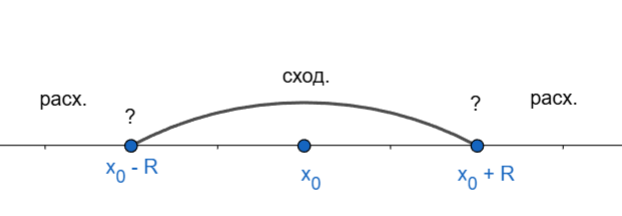
\includegraphics[width=0.4\textwidth]{addchapters1/images/addchapters1_2024_10_18_2}
        \end{wrapfigure}

        Для сдвинутого ряда $\sum_{n = 0}^\infty c_n (x - x_0)^n \quad \forall x: \ |x - x_0| < R$ - сходится; $\forall x: \ |x - x_0| > R$ - расходится
        
        Сходимость ряда в $x_0 \pm R$ нужно проверять специально

        \Nota Чаще всего исследование на сходимость проводится по признакам Даламбера, Коши

        \Ex $\sum_{n = 1}^\infty \frac{x^n}{n} (-1)^{n + 1}$

    \end{minipage}


    $\lim_{n \to \infty} \left|\frac{u_{n+1}}{u_n}\right| = \lim_{n \to \infty} \frac{1}{n + 1} |x|^{n + 1} \frac{n}{|x|^n} = \lim_{n \to \infty} |x| = |x| < 1$

    Предварительно $D = (-1; 1)$. 
    
    Далее, рассмотрим $x = \pm 1$: 
    
    $\quad (x = 1): \sum_{n = 1}^\infty \frac{(-1)^{n + 1}}{n}$ - сходится

    $\quad (x = -1): \sum_{n = 1}^\infty \frac{-1}{n}$ - расходится

    Итак, $D = (-1; 1]$

    \subsection{3. Ряд Тейлора}

    \Mem Формула Тейлора: $f(x) \in C^{n + 1}_{U_\delta (x_0)}$, тогда $f(x) \overset{x \in U_\delta (x_0)}{=\joinrel=\joinrel=} f(x_0) + 
    \frac{f^\prime (x_0)}{1!} (x - x_0) + \frac{f^{\prime\prime} (x_0)}{2!} (x - x_0)^2 + \dots + \frac{f^{(n)} (x_0)}{n!} (x - x_0)^n + \frac{f^{(n + 1)} (\xi)}{(n + 1)!} (x - x_0)^{n + 1}$

    Чтобы $f(x)$ в пределе равнялось $\sum_{n = 0}^\infty \frac{f^{(n)}(x_0)}{n!} (x - x_0)^n$, нужно, чтобы $r_n(x) \to 0$


\end{document}
